% =====================================================================
% Artigo (entregável M11) --- VERSÃO EM PORTUGUÊS, modular.
% Montado em 10/11/2026 a partir dos resultados REAIS do laboratório
% (fl-robustness-lab/results/). Figuras em figuras/ são geradas por
% gerar_figuras.py (dados auditados; ver dados/*.csv).
%
% Estrutura:
%   main.tex            -> preâmbulo + \input das seções
%   secoes/*.tex        -> uma seção por arquivo
%   figuras/*.pdf       -> figuras (vetoriais) geradas de dados reais
%   dados/*.csv         -> números por figura (reprodutibilidade)
%
% Para compilar no Overleaf: subir a pasta inteira (zip) e definir main.tex
% como documento principal. Trocar o documentclass pelo template da
% conferência-alvo quando definido. Lacunas restantes: \todo{...}.
% =====================================================================
\documentclass[10pt,conference]{article}
\usepackage[utf8]{inputenc}
\usepackage[T1]{fontenc}
\usepackage[brazil]{babel}
\usepackage[margin=1in]{geometry}
\usepackage{amsmath,amssymb}
\usepackage{graphicx}
\usepackage{booktabs}
\usepackage{xcolor}
\usepackage{subcaption}
\usepackage{hyperref}
\hypersetup{colorlinks=true,linkcolor=blue,citecolor=blue,urlcolor=blue}

\graphicspath{{figuras/}}
\newcommand{\todo}[1]{\textcolor{red}{[TODO: #1]}}

\title{Contenção de Backdoors com Seleção de Camadas em\\
Aprendizado Federado por Corroboração entre Camadas}
\author{Marcos G. O. Morais \quad Leandro A. Villas\\
\small Instituto de Computação, Universidade Estadual de Campinas (UNICAMP) --- H.IAAC\\
\small \texttt{\{marcos.morais, leandro.villas\}@ic.unicamp.br}}
\date{Rascunho --- \today}

\begin{document}
\maketitle

\begin{abstract}
Ataques de backdoor com seleção de camadas escondem o envenenamento em alguns poucos
tensores de parâmetros, de modo que agregadores robustos que atuam tensor a tensor não
conseguem isolá-lo. Reproduzimos fielmente o ataque mais recente dessa classe,
o LaySelFL (CVPR 2026), em seu próprio cenário (ResNet18-GN, CIFAR-10, 20 clientes, 6
maliciosos, Dirichlet $\alpha{=}0{,}9$, 205 rodadas) e mostramos que ele atinge uma taxa de
sucesso do backdoor (ASR) de $82\%$ sem defesa, enquanto \emph{toda a classe} de defesas
publicadas falha em contê-lo (Multi-Krum, AlignIns, FedSurrogate, FLAME, RFLDefense $70$--$88\%$;
a melhor, LASA, $21{,}7\%$). Diagnosticamos a falha --- o envenenamento vaza pelos tensores
convolucionais, onde cada tensor isolado permanece abaixo de qualquer limiar por tensor --- e
propomos uma defesa que \emph{corrobora evidências entre camadas}: um sinal por tensor ($z$
robusto do cosseno par a par de atualizações centradas na mediana, somado à norma da atualização)
é agregado contando quantos tensores acusam cada cliente, e um cliente confirmado por pelo menos
$T$ tensores é removido. Em quatro sementes, a família por corroboração contém o ataque (expurgo
do cliente $4{,}3\pm1{,}3\%$, substituição por consenso $5{,}5\pm2{,}0\%$, corte por tensor
$10{,}5\pm6{,}3\%$), generaliza para VGG19 e EfficientNet e para o gatilho adaptativo A3FL no
CIFAR-10 ($12{,}6\%$), e custa $\leq 6{,}5\%$ de tempo extra por rodada, sem dados limpos no
servidor. Caracterizamos o modelo de ameaça sob o qual a defesa se sustenta ($\geq 2$ atacantes
em conluio) e um adversário adaptativo que conhece a defesa.
\end{abstract}

\section{Introdução}
O aprendizado federado (FL) permite que clientes treinem um modelo compartilhado sem
compartilhar dados, mas o servidor agrega atualizações que não pode inspecionar, o que abre
caminho para ataques de backdoor. Uma família recente e perigosa é a de \emph{seleção de
camadas}: o atacante treina o backdoor em um subconjunto escolhido de camadas e mantém o
restante próximo de uma atualização benigna, de modo que agregadores robustos que atuam por
tensor não enxergam nada anômalo em nenhum tensor isolado. O LaySelFL (CVPR 2026) \cite{laysel}
é o estado da arte dessa família.

\paragraph{Contribuições.}
\begin{itemize}
  \item Reproduzimos o LaySelFL fielmente e mostramos que ele se fixa no topo ($82\%$ de ASR)
  onde \emph{seis} defesas publicadas --- incluindo a defesa cirúrgica de 2026, FedSurrogate ---
  falham (Seç.~\ref{sec:exp}, Fig.~\ref{fig:rigor}).
  \item Diagnosticamos a falha como um \emph{vazamento convolucional} e propomos a
  \emph{corroboração entre camadas}: decidir pelo cliente contando os tensores que o acusam,
  e não tensor a tensor (Seç.~\ref{sec:method}, Fig.~\ref{fig:corrob}).
  \item Mostramos a contenção com rigor estatístico (4 sementes), generalidade entre
  arquiteturas e sob o gatilho adaptativo A3FL, e baixo sobrecusto, sem dados limpos no
  servidor (Seç.~\ref{sec:exp}, Figs.~\ref{fig:geral} e~\ref{fig:overhead}).
  \item Enunciamos o modelo de ameaça ($\geq 2$ atacantes em conluio) e avaliamos um adversário
  adaptativo que conhece a regra de corroboração (Seç.~\ref{sec:adaptive}).
\end{itemize}

\section{Trabalhos Relacionados}\label{sec:related}
A agregação robusta contra clientes bizantinos/backdoor abrange regras baseadas em distância e
geometria (Multi-Krum \cite{krum}, FLAME \cite{flame}), regras baseadas em similaridade de
cosseno (FoolsGold, CosDefense, AlignIns) e regras por camada. Os ingredientes que usamos têm
precedentes isolados: cosseno de atualizações, corroboração entre camadas baseada em contagem
(FLD, 2023) e substituição cirúrgica por camada (FedSurrogate, 2026). Nossa originalidade é
\emph{empírica e diagnóstica}: mostramos que esta instanciação específica \emph{contém} os
ataques de seleção de camadas de 2026 que quebram toda a classe --- incluindo FedSurrogate e FLD,
que compartilham nosso mecanismo --- e diagnosticamos por que a classe falha.
\todo{expandir com citações/anos precisos a partir do documento de trabalhos relacionados.}

\section{Modelo de Ameaça e Configuração}\label{sec:setup}
\textbf{Modelo de ameaça.} Até $m$ dos $n$ clientes são maliciosos e estão em \emph{conluio}:
compartilham um objetivo de backdoor e enviam atualizações envenenadas semelhantes. O servidor
não tem dados rotulados (exceto um pequeno conjunto limpo usado apenas pela sonda opcional).
Assumimos $\geq 2$ atacantes em conluio; um único atacante isolado está fora do escopo do sinal
de corroboração (Seç.~\ref{sec:adaptive}).

\textbf{Cenário fiel (LaySelFL).} ResNet18-GN, CIFAR-10, 20 clientes (6 maliciosos), Dirichlet
$\alpha{=}0{,}9$, 205 rodadas, ataque ativo nas rodadas 80--200, gatilho BadNet, classe-alvo 4,
fração de envenenamento 0{,}2. Critério de sucesso fixado antes de rodar: uma defesa
\emph{contém} o ataque se a ASR final for $\leq 20\%$.

\section{Método: Corroboração entre Camadas}\label{sec:method}
Seja $\Delta_i=\theta_i-\theta_{\text{servidor}}$ a atualização achatada do cliente $i$,
fatiada por tensor de parâmetros $g$. Removemos o consenso centrando na mediana por coordenada,
$C_i=\Delta_i-\mathrm{median}_j(\Delta_j)$. Por tensor $g$, dois sinais descrevem o cliente $i$
em relação aos demais --- direção e norma:
\begin{equation}
s_g(i)=\max_{j\neq i}\cos\!\big(C_i[g],C_j[g]\big),\qquad n_g(i)=\lVert C_i[g]\rVert .
\end{equation}
Cada um é padronizado por um $z$ \emph{robusto} (mediana / MAD) entre os clientes, e o escore por
tensor sinaliza o cliente $i$ quando
\begin{equation}
z_g(i)=\max(z_{\text{sim}},0)+\max(z_{\text{norm}},0) > z_{\text{thr}}\;(=3).
\end{equation}

\textbf{Diagnóstico (vazamento convolucional).} Um agregador-sombra que apenas registra o sinal
(sem agir) mostra que, contra o LaySelFL, o atacante é sinalizado em $\approx 21$ tensores por
rodada (mediana; $p_{10}\approx12$), enquanto um cliente benigno é sinalizado em $\approx 1$
($p_{90}\approx7$) --- Fig.~\ref{fig:corrob}. O envenenamento está espalhado de forma rala por
muitos tensores convolucionais, de modo que decidir tensor a tensor descarta a evidência entre
tensores; é exatamente essa evidência agregada que separa os grupos.

\begin{figure}[t]\centering
  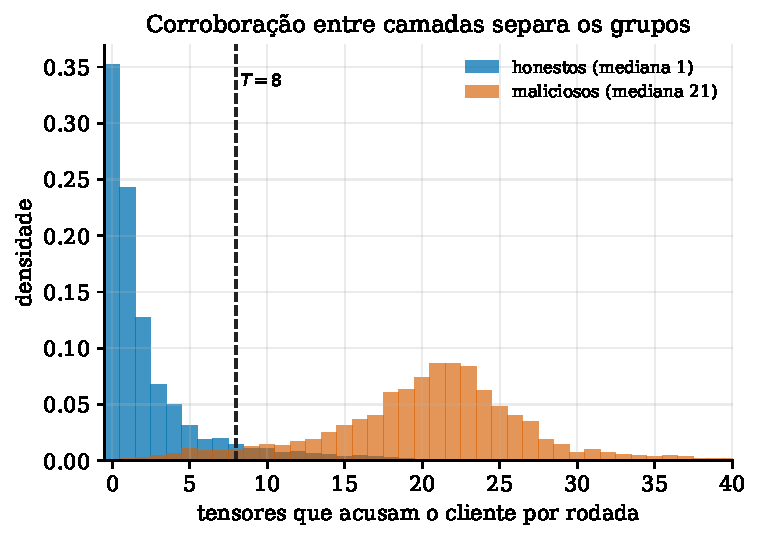
\includegraphics[width=\linewidth]{fig_corroboracao.pdf}
  \caption{Agregador-sombra no cenário fiel (4 sementes, rodadas de ataque 80--200): número de
  tensores que acusam cada cliente por rodada. Honestos concentram-se em $\approx 1$; maliciosos,
  em $\approx 21$. A decisão tensor a tensor joga fora essa separação.}
  \label{fig:corrob}
\end{figure}

\textbf{Corroboração.} Por isso \emph{contamos} os tensores que acusam e decidimos pelo cliente:
\begin{equation}
\text{contagem}_i=\sum_g [\,z_g(i)>z_{\text{thr}}\,],\qquad \text{confirmado se } \text{contagem}_i\geq T .
\end{equation}
A curva de detecção sobre $T$ (Fig.~\ref{fig:curvaT}) dá $F_1=0{,}88$ em $T{=}8$ (revocação
$0{,}95$, precisão $0{,}82$), com pico em $F_1=0{,}90$ ($T{=}12$). \textbf{A resposta} é modular:
remover o cliente confirmado de todos os tensores (\emph{corr}); expurgar completamente qualquer
cliente sinalizado (\emph{client}); ou substituir a contribuição suspeita pela mediana benigna,
preservando a massa de votos (\emph{corr-soft}).

\begin{figure}[t]\centering
  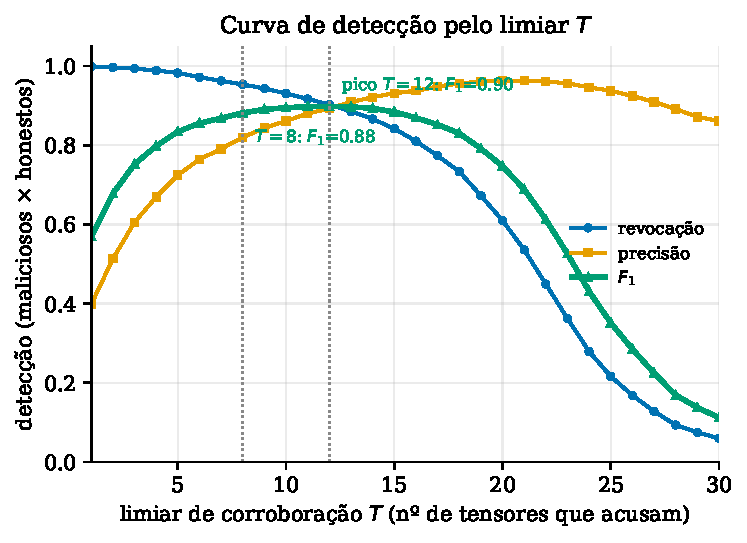
\includegraphics[width=0.92\linewidth]{fig_curva_T.pdf}
  \caption{Detecção de clientes maliciosos pelo limiar de corroboração $T$ (média de 4 sementes).
  Um patamar largo de $F_1$ alto ($T\in[6,16]$) torna a escolha de $T$ pouco sensível.}
  \label{fig:curvaT}
\end{figure}

\section{Experimentos}\label{sec:exp}
\textbf{Resultado principal (rigor estatístico, 4 sementes).} A Tabela~\ref{tab:rigor} e a
Fig.~\ref{fig:rigor} reportam a ASR final do backdoor (média$\pm$desvio-padrão sobre as sementes
42--45). Nossa família por corroboração contém o ataque; as seis defesas publicadas falham em
todas as sementes. A LASA pareceu conter com uma única semente ($13{,}5\%$) --- foi sorte da
semente.

\begin{figure}[t]\centering
  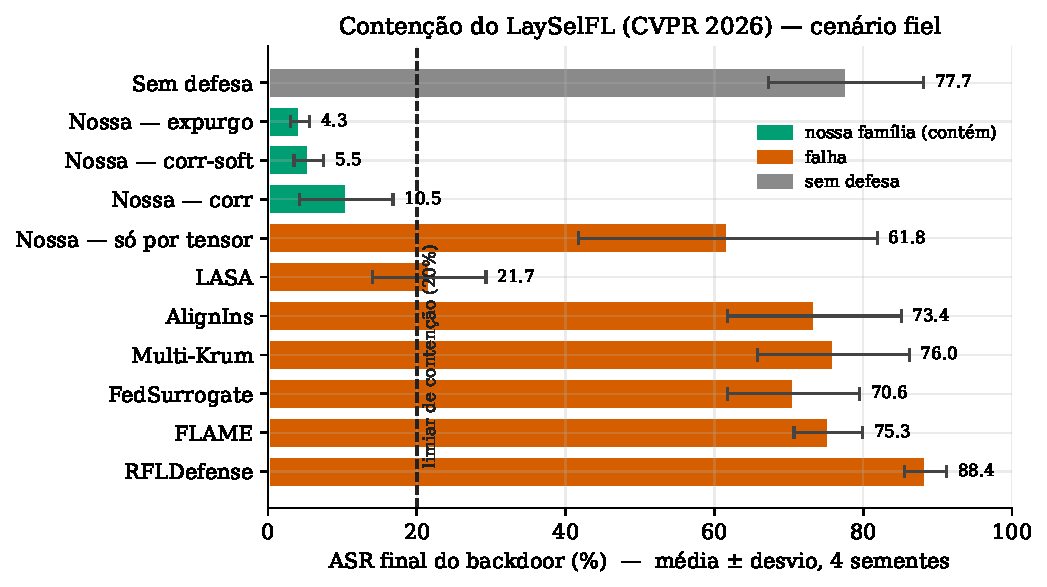
\includegraphics[width=\linewidth]{fig_rigor_asr.pdf}
  \caption{ASR final do backdoor no cenário fiel do LaySelFL (11 agregações, 4 sementes). Nossa
  família (verde) fica muito abaixo do limiar de contenção de 20\%; todas as defesas publicadas
  (laranja) falham. ``Nossa --- só por tensor'' mostra que agir tensor a tensor, sem corroborar,
  não basta.}
  \label{fig:rigor}
\end{figure}

\begin{table}[t]\centering\small
\caption{ASR final do backdoor, cenário fiel do LaySelFL, 11 agregações $\times$ 4 sementes.}
\label{tab:rigor}
\begin{tabular}{lcc}
\toprule
Agregação & ASR (4 sementes) & Contém? \\
\midrule
Sem defesa (referência) & $77{,}7\pm10{,}4\%$ & --- (ataque se fixa) \\
\textbf{Nossa --- expurgo do cliente} & $\mathbf{4{,}3\pm1{,}3\%}$ & sim \\
\textbf{Nossa --- consenso (corr-soft)} & $\mathbf{5{,}5\pm2{,}0\%}$ & sim \\
\textbf{Nossa --- corte por tensor (corr)} & $\mathbf{10{,}5\pm6{,}3\%}$ & sim (3/4) \\
Nossa --- apenas por tensor (sn) & $61{,}8\pm20{,}1\%$ & não \\
LASA & $21{,}7\pm7{,}6\%$ & não \\
AlignIns & $73{,}4\pm11{,}7\%$ & não \\
Multi-Krum & $76{,}0\pm10{,}2\%$ & não \\
FedSurrogate & $70{,}6\pm8{,}9\%$ & não \\
FLAME & $75{,}3\pm4{,}6\%$ & não \\
RFLDefense & $88{,}4\pm2{,}8\%$ & não \\
\bottomrule
\end{tabular}
\end{table}

\textbf{Generalidade.} A Fig.~\ref{fig:geral} estende o resultado a outras arquiteturas e ao
gatilho adaptativo. O ataque se fixa na VGG19 ($95{,}6\%$) e na EfficientNet ($85{,}3\%$); nossa
família contém na VGG19 ($9{,}2\%$, \emph{corr} $T{=}2$) e na EfficientNet ($13{,}0\%$,
\emph{corr-soft} $T{=}2$), confirmando a regra ``corroboração mais fraca $\Rightarrow$ expurgo mais
agressivo''.

\begin{figure}[t]\centering
  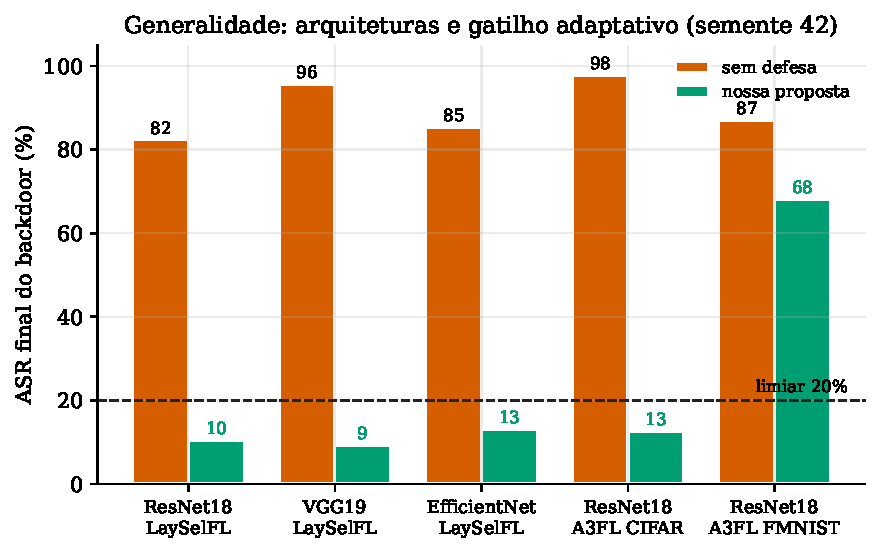
\includegraphics[width=\linewidth]{fig_generalidade.pdf}
  \caption{Generalidade (semente 42): ASR sem defesa (laranja) vs.\ nossa melhor variante (verde).
  A contenção se mantém em quatro dos cinco casos; a exceção (A3FL no FMNIST) é discutida na
  Seç.~\ref{sec:limits}.}
  \label{fig:geral}
\end{figure}

\textbf{Gatilho adaptativo (A3FL).} Sob o gatilho adversarialmente adaptativo A3FL \cite{a3fl}, o
ataque se fixa no CIFAR-10 ($97{,}7\%$) e nossa variante \emph{corr} o contém ($12{,}6\%$). O caso do
FMNIST ($68{,}2\%$) é uma assimetria conhecida sob investigação (Seç.~\ref{sec:limits}).

\textbf{Sobrecusto.} O agente adiciona $\leq 6{,}5\%$ de tempo por rodada em relação ao FedAvg
(Fig.~\ref{fig:overhead}), uma ordem de grandeza abaixo das defesas baseadas em busca
geométrica (LASA, AlignIns, RFLDefense), que chegam a $50$--$93\%$ na VGG19.

\begin{figure}[t]\centering
  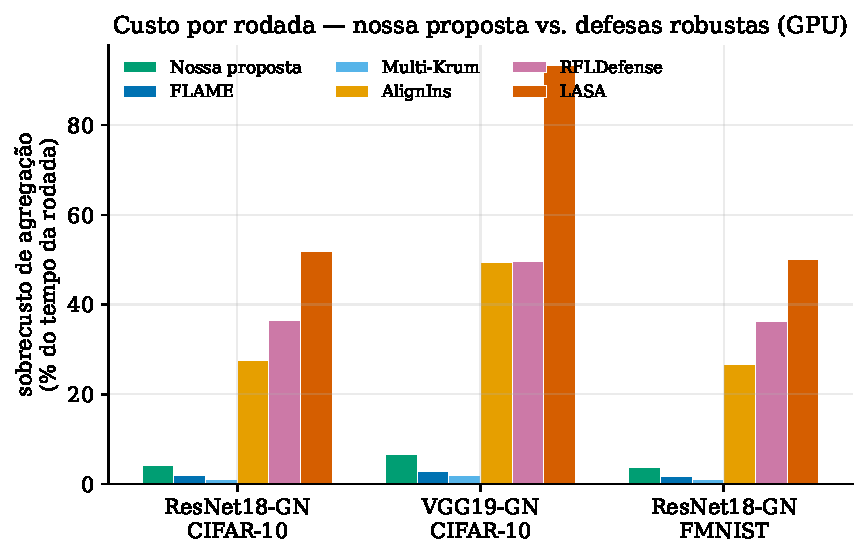
\includegraphics[width=\linewidth]{fig_overhead.pdf}
  \caption{Sobrecusto de agregação por rodada (\% do tempo de treino da rodada, em GPU). Nossa
  proposta fica junto das defesas mais baratas (FLAME, Multi-Krum) e muito abaixo das baseadas em
  busca geométrica.}
  \label{fig:overhead}
\end{figure}

\textbf{Sensibilidade ao limiar $T$.} Fixamos $T{=}8$ antes de rodar, a partir da curva de detecção
(Fig.~\ref{fig:curvaT}), medida sem retreinar o modelo. Para verificar se essa escolha depende de
ajuste fino, retreinamos a variante \emph{corr} com $T\in\{4,11,14\}$ nas sementes 42--44, sem mudar
mais nada (Tabela~\ref{tab:sensT}). Todos os valores testados reduzem o ataque de $83{,}2\%$ para
$11{,}5$--$17{,}1\%$ em média, o que confirma o patamar largo da curva de detecção. Os extremos
mostram os dois lados do compromisso: com $T{=}4$ o expurgo fica mais agressivo, custa $2{,}4$\,pp de
acurácia em relação a $T{=}8$ e, ainda assim, não contém a semente 44 ($28{,}3\%$); com $T{=}14$ a
detecção perde revocação e a ASR média sobe para $17{,}1\%$, com duas sementes perto do limiar de
$20\%$. O melhor resultado ficou em $T{=}11$ ($11{,}5\pm1{,}4\%$, contém nas 3 sementes), perto do
pico de $F_1$ da curva ($T{=}12$). Mantemos $T{=}8$, fixado antes, e reportamos a varredura como
evidência de que o resultado não depende de calibrar $T$ com o ataque conhecido.

\begin{table}[t]\centering\small
\caption{Sensibilidade ao limiar $T$ (variante \emph{corr}, cenário fiel do LaySelFL, sementes 42--44).
ASR final e acurácia final em \%; ``contém'' = ASR final $\leq 20\%$.}
\label{tab:sensT}
\begin{tabular}{lcccc}
\toprule
$T$ & ASR (s42 / s43 / s44) & ASR média & Contém & Acurácia \\
\midrule
4 & $5{,}9$ / $5{,}9$ / $28{,}3$ & $13{,}4\pm13{,}0$ & 2/3 & $70{,}8$ \\
\textbf{8 (fixado antes)} & $7{,}9$ / $7{,}6$ / $21{,}4$ & $12{,}3\pm7{,}9$ & 2/3 & $73{,}2$ \\
11 & $10{,}7$ / $10{,}7$ / $13{,}1$ & $11{,}5\pm1{,}4$ & 3/3 & $73{,}6$ \\
14 & $18{,}2$ / $19{,}9$ / $13{,}2$ & $17{,}1\pm3{,}5$ & 3/3 & $73{,}8$ \\
Sem defesa & $82{,}3$ / $78{,}1$ / $89{,}2$ & $83{,}2$ & 0/3 & $75{,}5$ \\
\bottomrule
\end{tabular}
\end{table}

\textbf{Custo sem ataque (falsos positivos).} Sob ataque, a precisão da detecção em $T{=}8$ é
$0{,}82$, ou seja, alguns honestos também são confirmados. Para medir o custo disso, repetimos o
cenário fiel com todos os 20 clientes honestos (mesma partição de dados, janela de ataque nunca
iniciada), em $\alpha{=}0{,}9$, o cenário do LaySelFL, e em $\alpha{=}0{,}1$, com dados muito mais
heterogêneos (Tabela~\ref{tab:fp}). Nenhuma variante cria backdoor: a ASR do gatilho fica em
$1{,}5$--$7{,}8\%$, o mesmo nível do modelo sem defesa ($6{,}1$--$6{,}7\%$). O custo de acurácia
separa as variantes. A \emph{corr-soft} é a mais barata ($-1{,}8$\,pp em $\alpha{=}0{,}9$ e $-3{,}0$\,pp
em $\alpha{=}0{,}1$), porque troca a contribuição suspeita pelo consenso em vez de descartá-la. A
\emph{client}, que descarta qualquer cliente acusado por um único tensor, retira em média 10 dos 20
clientes por avaliação e perde $5{,}2$\,pp em $\alpha{=}0{,}9$ e $13{,}8$\,pp em $\alpha{=}0{,}1$. Por
isso recomendamos a \emph{corr-soft} no caso geral e reservamos a \emph{client} para ameaça alta.

\begin{table}[t]\centering\small
\caption{Custo sem ataque (semente 42; 20 clientes honestos). Acurácia final em \%; $\Delta$ em
relação à agregação sem defesa; ``descartados'' = honestos confirmados por avaliação (média).}
\label{tab:fp}
\begin{tabular}{lcccc}
\toprule
& \multicolumn{2}{c}{$\alpha{=}0{,}9$} & \multicolumn{2}{c}{$\alpha{=}0{,}1$} \\
Agregação & Acurácia ($\Delta$) & Descartados & Acurácia ($\Delta$) & Descartados \\
\midrule
Sem defesa & $76{,}7$ & 0 & $67{,}9$ & 0 \\
\textbf{corr-soft} & $74{,}8$ ($-1{,}8$) & $1{,}6$ & $64{,}9$ ($-3{,}0$) & $2{,}8$ \\
corr & $74{,}5$ ($-2{,}2$) & $2{,}0$ & $63{,}8$ ($-4{,}2$) & $3{,}2$ \\
client & $71{,}5$ ($-5{,}2$) & $10{,}2$ & $54{,}2$ ($-13{,}8$) & $7{,}8$ \\
\bottomrule
\end{tabular}
\end{table}

\textbf{CIFAR-100.} Repetimos o cenário fiel no CIFAR-100, com 100 classes, nas sementes 42 e 43
(Tabela~\ref{tab:c100}). O ataque se fixa ($33{,}4$ e $45{,}0\%$ de ASR final; picos de $51$ a $58\%$)
e as três variantes o contêm por completo ($0{,}0$--$0{,}2\%$ de ASR final, pico máximo de $1{,}2\%$).
A acurácia do modelo limpo, treinado sem ataque e sem defesa, é $44{,}6\%$; a \emph{corr} e a
\emph{corr-soft} perdem de $2{,}3$ a $3{,}1$\,pp em relação à agregação sem defesa, e a \emph{client}
perde $6{,}7$ a $11{,}4$\,pp. Ao contrário do CIFAR-10, aqui a LASA também contém ($0{,}1$--$0{,}2\%$),
com custo semelhante ao nosso; FedSurrogate ($34$--$44\%$) e FLAME ($57$--$69\%$) falham. O CIFAR-100,
portanto, mostra que a contenção se mantém com muitas classes, mas não diferencia a nossa proposta
da LASA; a diferença entre as duas está no CIFAR-10, onde a LASA contém em apenas 2 de 6 sementes.

\begin{table}[t]\centering\small
\caption{CIFAR-100, cenário fiel (ResNet18-GN, 20 clientes, 6 maliciosos), sementes 42 e 43. Valores
em \%. Modelo limpo (sem ataque): acurácia $44{,}6\%$, ASR do gatilho $0{,}1\%$.}
\label{tab:c100}
\begin{tabular}{lccc}
\toprule
Agregação & ASR final (s42 / s43) & Pico da ASR & Acurácia \\
\midrule
Sem defesa & $33{,}4$ / $45{,}0$ & $51{,}1$ / $57{,}7$ & $43{,}3$ / $44{,}8$ \\
\textbf{corr-soft} & $0{,}2$ / $0{,}1$ & $0{,}3$ / $0{,}4$ & $40{,}2$ / $42{,}0$ \\
\textbf{corr} & $0{,}2$ / $0{,}2$ & $0{,}2$ / $0{,}6$ & $40{,}6$ / $42{,}5$ \\
\textbf{client} & $0{,}0$ / $0{,}2$ & $0{,}2$ / $1{,}2$ & $31{,}9$ / $38{,}1$ \\
LASA & $0{,}2$ / $0{,}1$ & $0{,}2$ / $0{,}3$ & $40{,}9$ / $42{,}8$ \\
FedSurrogate & $34{,}1$ / $43{,}5$ & $49{,}3$ / $59{,}9$ & $43{,}0$ / $44{,}5$ \\
FLAME & $57{,}0$ / $68{,}8$ & $75{,}3$ / $83{,}7$ & $37{,}0$ / $38{,}1$ \\
\bottomrule
\end{tabular}
\end{table}

\section{Adversário Adaptativo (conhece a defesa)}\label{sec:adaptive}
Avaliamos um atacante onisciente que conhece a regra de corroboração, o limiar $T$ e as
atualizações honestas da rodada. Ele (A) concentra o envenenamento em $m$ tensores --- revertendo
os demais tensores sensíveis para sua própria atualização benigna, para que não sinalizem --- e (B)
dessincroniza os clientes maliciosos com ruído independente, de modo que o cosseno mútuo caia; ele
varre $(m,\nu)$ para encontrar o backdoor mais forte que mantém a contagem de corroboração abaixo de
$T$. A hipótese sob teste (H4) é que há uma tensão fundamental: reduzir $m$ para escapar da contagem
também reduz a fração de parâmetros do backdoor, enfraquecendo o ataque.
\textbf{Resultado.} O atacante adaptativo vence a corroboração (Tabela~\ref{tab:adapt}, sementes 42--47):
a ASR final é $62{,}5\%$ contra a \emph{corr} e $53{,}5\%$ contra a \emph{corr-soft}, ante $83{,}4\%$ sem
defesa com o mesmo ataque concentrado. A \emph{client} resiste mais ($25{,}0\%$ em média), mas é instável
(de $6{,}0$ a $58{,}5\%$ entre sementes) e perde $8{,}4$\,pp de acurácia. A hipótese H4 se confirma só em
parte: o atacante raramente consegue deixar \emph{todos} os maliciosos abaixo de $T$ na mesma rodada
($1$--$3\%$ das rodadas), mas não precisa disso. Em $37\%$ dos pares (atacante, rodada) contra a
\emph{corr-soft}, um malicioso fica abaixo de $T$ e entra na agregação sem ser confirmado; o veneno passa
aos poucos, por dois ou três atacantes a cada rodada, e o backdoor se acumula.

\textbf{O custo imposto ao atacante.} A defesa não impede o ataque, mas o encarece. Contra a
\emph{corr-soft}, o backdoor leva o dobro do tempo para pegar: chega a $50\%$ na rodada $165$, ou seja,
$85$ rodadas depois do início do ataque, contra $43$ rodadas sem defesa; a ASR média durante o ataque
cai de $62{,}1$ para $37{,}7\%$; a final, de $83{,}4$ para $53{,}5\%$ ($-30$\,pp). Contra a \emph{client},
o ataque só passa de $20\%$ por volta da rodada $167$ e, em 5 das 6 sementes, nunca chega a $50\%$.

\begin{table}[t]\centering\small
\caption{Atacante adaptativo ciente da corroboração, cenário fiel do LaySelFL, sementes 42--47 (médias).
O ataque começa na rodada 80. Valores de ASR e acurácia em \%.}
\label{tab:adapt}
\begin{tabular}{lccccc}
\toprule
Agregação & ASR final & ASR média no ataque & ASR $\geq 50\%$ na rodada & Acurácia \\
\midrule
Sem defesa (ataque concentrado) & $83{,}4$ & $62{,}1$ & $123$ & $76{,}8$ \\
corr & $62{,}5$ & $43{,}3$ & $155$ & $74{,}8$ \\
\textbf{corr-soft} & $53{,}5$ & $37{,}7$ & $165$ & $74{,}5$ \\
client & $25{,}0$ & $15{,}5$ & $180$ (5 de 6 nunca) & $68{,}4$ \\
\bottomrule
\end{tabular}
\end{table}

\textbf{Respostas testadas.} Aplicar uma agregação robusta depois da corroboração não resolveu, contra um
atacante que também conhece essa agregação (sementes 42--45): com corte de norma por tensor a ASR final
fica em $60{,}2\%$ e com média aparada em $72{,}5\%$. Um atacante intermediário, que conhece a regra da
contagem mas não simula a agregação, chega a $62{,}8\%$ contra o corte de norma. Duas variantes que atacam
diretamente o vazamento abaixo de $T$ --- peso gradual em função da contagem e $T$ sorteado em segredo a
cada rodada --- estão em avaliação. \todo{inserir resultado da Fase 20.}

\section{Limitações}\label{sec:limits}
(i) O sinal precisa de $\geq 2$ atacantes em conluio; um atacante solitário é indistinguível pela
similaridade mútua. Validamos esse limite no repositório original do LP \cite{lp}: com 20\% de
maliciosos (2 por rodada) nossa proposta zera o backdoor ($0{,}1$--$0{,}3\%$), mas com 10\% (1 por
rodada) não defende ($\approx 72\%$). \todo{inserir a Fig.\ da Fase 9A: contagem de corroboração de
1 atacante $\approx$ benigno vs.\ 2 atacantes $\gg$ benigno (instrumentada; entra com GPU livre).}
(ii) O A3FL no FMNIST ainda não é contido ($68\%$, Fig.~\ref{fig:geral}); variantes de expurgo
agressivo estão em avaliação. (iii) O limiar de contagem $T$ precisa ser reduzido em arquiteturas com
corroboração mais fraca; a calibração automática (p.ex.\ via predição conformal) é trabalho futuro.

\section{Conclusão}
Uma classe de backdoors com seleção de camadas que derrota a agregação robusta por tensor ---
incluindo as defesas cirúrgicas de 2026 --- é contida corroborando o sinal por camada entre tensores
antes de decidir pelo cliente. O resultado se sustenta com rigor estatístico, entre arquiteturas e sob
um gatilho adaptativo, a baixo custo e sem dados limpos no servidor.

\begin{thebibliography}{9}
\bibitem{laysel} Li et al. Eliminate Distance Differences Induced by Backdoor Attacks: Layer-Selective
Training and Clipping to Mask Backdoor Models (LaySelFL). CVPR, 2026.
\bibitem{a3fl} Zhang et al. A3FL: Adversarially Adaptive Backdoor Attacks to Federated Learning. NeurIPS, 2023.
\bibitem{lp} Zhuang et al. Backdoor Federated Learning by Poisoning Backdoor-Critical Layers. ICLR, 2024.
\bibitem{krum} Blanchard et al. Machine Learning with Adversaries: Byzantine Tolerant Gradient Descent. NeurIPS, 2017.
\bibitem{flame} Nguyen et al. FLAME: Taming Backdoors in Federated Learning. USENIX Security, 2022.
\todo{adicionar FLD (2023), FedSurrogate (2026), AlignIns (2025), LASA (2025), RFLDefense com refs completas.}
\end{thebibliography}


\end{document}
